\newchapter{phaseMons}{Phase Monitor Performance}

This is the introductory text.

Mon1 = first mon in CT
Mon2 = second mon in CT
Mon3 = mon in TBL

Mon1/Mon2 = upstream phase
Mon3 = downstream phase

\newsection{monElectronics}{Phase Monitor Electronics}

Hybrid - remove dipole (position dependent) mode. 19dB below monopole mode for 1mm offset (11\% amplitude). 1mm beam offset = 2.8 degrees phase offset. 180 degree hybrids to remove. Additional 20 dB attenuation in dipole mode.

Bunch length sensitivity: more sensitive to variation in bunch length for longer variations. 5mm bunch length - 50\% amplitude output compared to 0mm. With 1mm bunches 16\% variation in bunch length needed to cause 1\% change in output voltage.

LO should have 5fs stability? What is the source of the LO?

Mixer output
\begin{align}
RF(t) &= A_{RF}(t)\cos[\omega_{RF} t + \phi(t)] \\
LO(t) &= A_{LO}\cos[\omega_{LO} t]
\end{align}
mixer multiplies
\begin{align}
\mathrm{Mixer}(t) &= RF(t) \times LO(t) \\
\mathrm{Mixer}(t) &= A_{RF}(t)A_{LO}\cos[\omega_{RF} t + \phi(t)]\cos[\omega_{LO} t]
\end{align}
trig identities
\begin{equation}
\mathrm{Mixer}(t) = \frac{A_{RF}(t)A_{LO}}{2}\left\lbrace\cos[(\omega_{LO} + \omega_{RF})t + \phi(t)] + \cos[(\omega_{LO} - \omega_{RF})t + \phi(t)]\right\rbrace
\end{equation}
filter high frequency
\begin{equation}
\mathrm{Mixer}(t) = \frac{A_{RF}(t)A_{LO}}{2}\cos[(\omega_{LO} - \omega_{RF})t + \phi(t)]
\label{e:mixOutAnyFreq} 
\end{equation}
LO frequency and RF frequency are the same
\begin{equation}
\mathrm{Mixer}(t) = \frac{A_{RF}(t)A_{LO}}{2}\cos[\phi(t)]
\label{e:mixOutSameFreq} 
\end{equation}
Diode used to measure \(A_{RF}\)
\begin{equation}
\mathrm{Diode}(t) = A_{RF}(t)^2
\end{equation}
The phase can be reconstructed by
\begin{align}
&\frac{\mathrm{Mixer}(t)}{\sqrt{\mathrm{Diode}(t)}} = A\cos[\phi(t)] \label{e:mixOverSqrtDio} \\
&\phi(t) = \arccos\left[\frac{\mathrm{Mixer(t)}}{A\sqrt{\mathrm{Diode(t)}}}\right]
\label{e:phaseRecIdeal} 
\end{align}

Beam/monitor frequency is 11.994 GHz.

Performance limited by:
Device non-linearity -- normally better for lower input power
Signal to noise -- better for high power
Therefore, split signal to 8 mixers -- low input power to each one -- to reduce effect of non-linearities. Then sum up results of each mixer to improve signal to noise.

Monitor -> attenuator? -> Hybrid sum -> attenuator? -> attenuator in gallery -> mixer RF input
LO -> phase shifter -> multiplier -> amplifier -> mixer LO input
Mixer output -> attenuator -> amplifier -> SiS OR -> attenuator->FONT
Diode output -> SiS/FONT

Latest power measurements:
Mon1 24.6 dBm + 3dB
Mon2 26.8 dBm + 3dB
Mon3 24.5 dBm
LO1 22.6 dBm
LO2 23.6 dBm
LO3 25.5 dBm

\newsection{sinFitAlgorithm}{Fitting Method}

Due to the dependence of the mixer output on \(\cos(\phi)\) as seen in the previous section, many of the measurements in this chapter require a sinusoidal fit of the form:
\begin{equation}
y = A\sin(bx + c) + d
\label{e:generalSinEq}
\end{equation}
The use of sine rather than cosine makes no difference to the fitted amplitude, \(A\), and offset, \(d\) which are usually the only parameters of interest in this chapter. It is also convenient to consider a mixer output of zero to correspond to zero phase (rather than \(90^\circ\) as in Equation~\ref{e:mixOverSqrtDio}). All the fits of this type have been performed using a weighted nonlinear least squares fit implemented in MatLab fitting libraries \cite{MatLabFit}. Each data point is weighted by the inverse of its standard error squared.

Care must be taken to select suitable initial values for the four parameters in the fit in order to avoid local minima and ensure a reasonable fit. This is particularly important for a sinusoidal fit as there are many solutions with different frequencies and phase offsets that can match the data. The frequency, \(b\), is the most critical parameter but for all the applications in this chapter this is already known, e.g. from the properties of the used phase shifters. Initial values for the three reamining parametrs are estimated as follows:
\begin{align}
A &= \frac{\mathrm{max}(y)-\mathrm{min}(y)}{2} \\
d &= \frac{\mathrm{max}(y)+\mathrm{min}(y)}{2} \\
c &= \arcsin\left(\frac{y-d}{A}\right) - bx
\end{align}
The initial amplitude, \(A\), and offset, \(d\), of the sine curve are simply determined by comparing the minimum and maximum output. These initial estimates are therefore highly biased by any large outliers around the minimum and maximum output, but this is rarely the case for the application here and these simple estimators are sufficient.
Rearranging Equation~\ref{e:generalSinEq} gives the expression for \(c\) above. Due to its use of arcsin the equation is only valid in the first and fourth quadrants, between \(-\pi/2\) and \(+\pi/2\) where the gradient of the sine curve is positive. The \(y\) value at each data point is compared to its neighbours to determine whether it is on the rising slope. The initial value of \(c\) is the mean value calculated across all the data points that meet this criteria.

Figure~\ref{f:sinFitEx} and Table~\ref{t:sinFitEx} show the results of an example fit using this approach. An initial distribution of points with \(y=\sin(x+1)+1\) is used (\(A = b = c = d = 1\)), with random noise added. \(b\) is assumed to be known, as is normal. The initial estimates for \(A\) and \(d\) are within a few percent of their true value. The initial estimate for \(c\) is within \(20\%\) of the correct value. After fitting all four parameters are in agreement with the expected values within error bars.

\begin{figure}
  \centering
  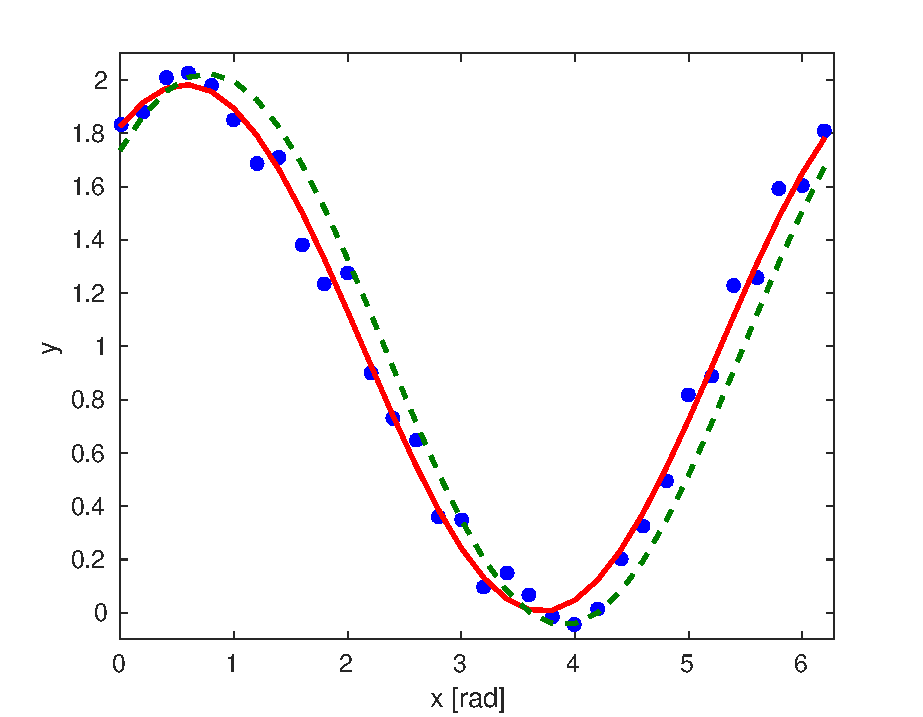
\includegraphics[width=0.9\textwidth]{Figures/phaseMons/sinFitEx}
  \caption{Example sine fit to generated data with added random noise.}
  \label{f:sinFitEx}
\end{figure}

\begin{table}
  \begin{center}
    \begin{tabular}{|c c c c|}
	   \hline
       Parameter & Value & Initial & Fit \\ \hline
       \(A\) & 1 & 1.03 & \(0.99\pm0.02\)\\
       \(b\) & 1 & 1 & \(1.00\pm0.02\) \\
       \(c\) & 1 & 0.81 & \(1.00\pm0.06\) \\
       \(d\) & 1 & 0.99 & \(0.99\pm0.02\) \\ \hline
    \end{tabular}
    \caption{Typical upstream phase and energy conditions at CTF3.}
  	\label{t:sinFitEx}
  \end{center}
\end{table}

\newsection{monSigResponse}{Signal Generator Measurements}

Measurements have been taken using a 12~GHz signal generator to determine the performance of the three sets of phase monitor electronics independently from the phase monitors themselves. In particular, these tests were focused on identifying the saturation and cross-talk characteristics of the output mixer and diode signals in order to determine a suitable input power range to use during normal operation.

\subsection{Experimental Setup}
\label{ss:sigGenSetup}

Two changes were made to the setup shown in Figure~[REF] for these tests. Firstly, the beam induced signal from the phase monitors usually connected to the RF port of the mixers is replaced by the output from a 12~GHz signal generator. To be able to reach the same input power levels as the beam signals the signal generator output is amplified using a [TODO:amplifierInfo]. This allows the input power to the mixers to be varied in a wide range between 0 and 33dBm, or between 0.2 and 10.0~V in terms of voltage. The precise power sent to the mixer is verified between each measurement using a power meter. 

Secondly, the diode outputs were amplified during these tests (using the same amplifier introduced in Section~\ref{ss:sisNoise}) by a factor 10 in voltage to reduce digitiser noise in the measurement. The non-amplified peak diode output is therefore 170~mV, rather than the 1.7~V seen in the plots in this section. The \(\pm500\)~mV mixer outputs have not been amplified. Usually the mixer output is amplified and the diode not amplified, as in Figure~[REF], for reasons that will become clear later in this chapter.

There are some differences between the properties of the generated signal and the beam signal that would be used in normal operation. Firstly, unlike the pulsed beam signal the used generated signal is continuous. It has been verified that the response of the mixers is equivalent for both the continuous and pulsed signals, at least in terms of output power and saturation levels [REF]. The cross-talk properties are difficult to characterise with beam based measurements alone, but assumed to be similar.

Secondly, the phase of the generated signal does not vary with time, compared to the beam signal which has a large \(\sim40^\circ\) phase sag along the pulse and much larger phase jitter. If the signal generator was used at the same frequency as the beam and LO signals, 11.994~GHz, the mixer output would therefore be constant as it depends only on the static phase as per Equation~\ref{e:mixOutSameFreq}. Instead, a generated signal with a slightly lower frequency of 11.991~GHz has been used. From Equation~\ref{e:mixOutAnyFreq} it can be seeen that in this case the mixer output voltage is sinusoidal, with a frequency equal to the frequency difference between the LO and RF inputs -- or \(11.994-11.991\)~GHz = 3~MHz with the setup used here. This has the benefit of being able to see the response of the electronics to all input phases in one measurement, rather than having to take multiple measurements varying the LO phase shifter between each one.

\subsection{Results}
\label{ss:sigGenResults}

Figures~\ref{f:sigGenAllMix1}--\ref{f:sigGenAllDio3} show the mixer and diode outputs for all three sets of electronics at each of the input power levels sent from the signal generator. These will be referred back to and discussed in more detail in later sections. All mixer outputs show a sinusoidal oscillation with a frequency of 3~MHz, or 60 samples at the sampling frequency of 192~MHz. Fits to the mixer response are presented in Section~\ref{ss:sigGenMixFit}. An oscillation with the same frequency is also visible on the diode outputs, with the largest amplitude for the 2nd set of electronics. This is not ideal and is discussed in Section~\ref{ss:crossTalk}. Finally, output of the mixer and diode increases with the input power, as expected. At high input powers the outputs begin to saturate. This is apparent by observing the diode signals, on which the output is much flatter at the highest power levels, without the oscillation seen at low input powers. This is discussed in Section~\ref{ss:monSaturation}.

\begin{figure}
  \centering
  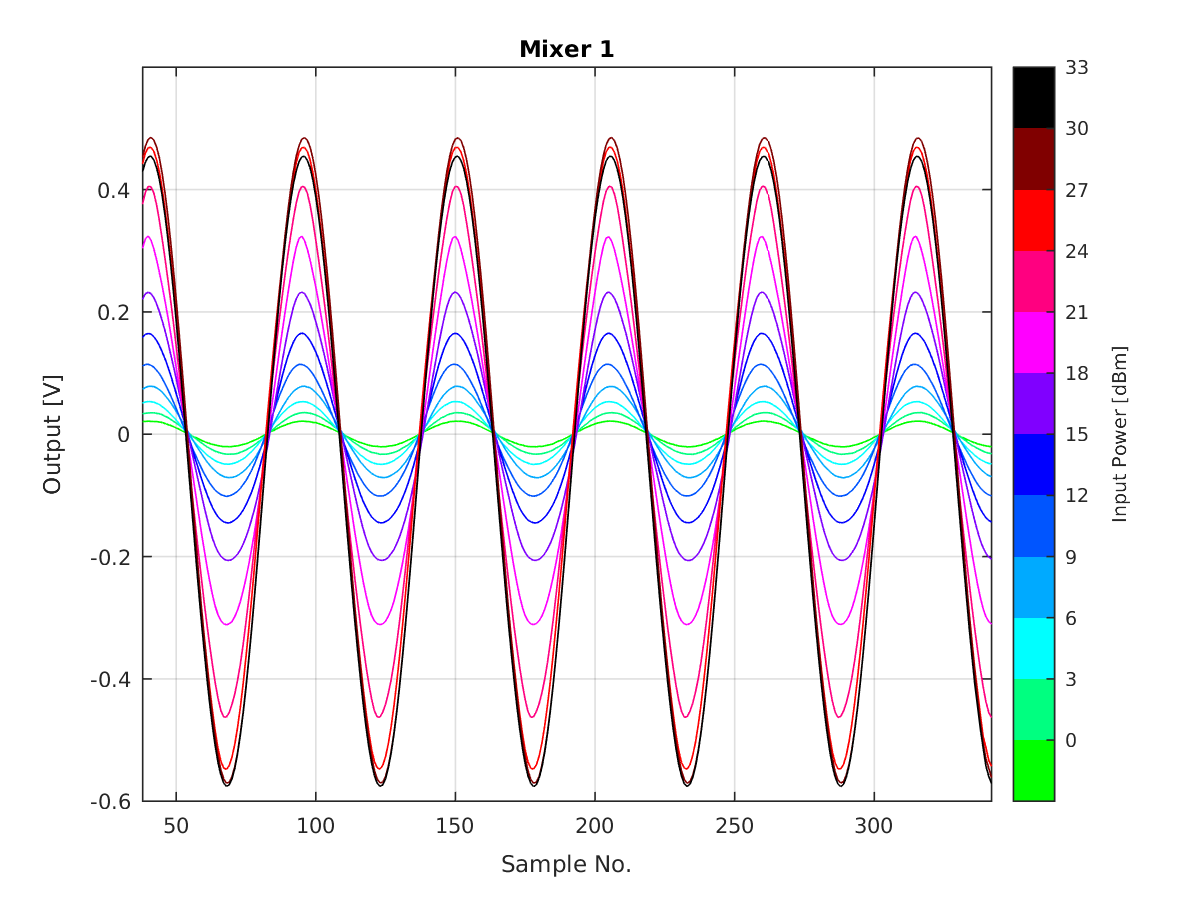
\includegraphics[width=0.9\textwidth]{Figures/phaseMons/Mixer1_AllPowerLevels}
  \caption{Response of Mixer 1 to signal generator input.}
  \label{f:sigGenAllMix1}
  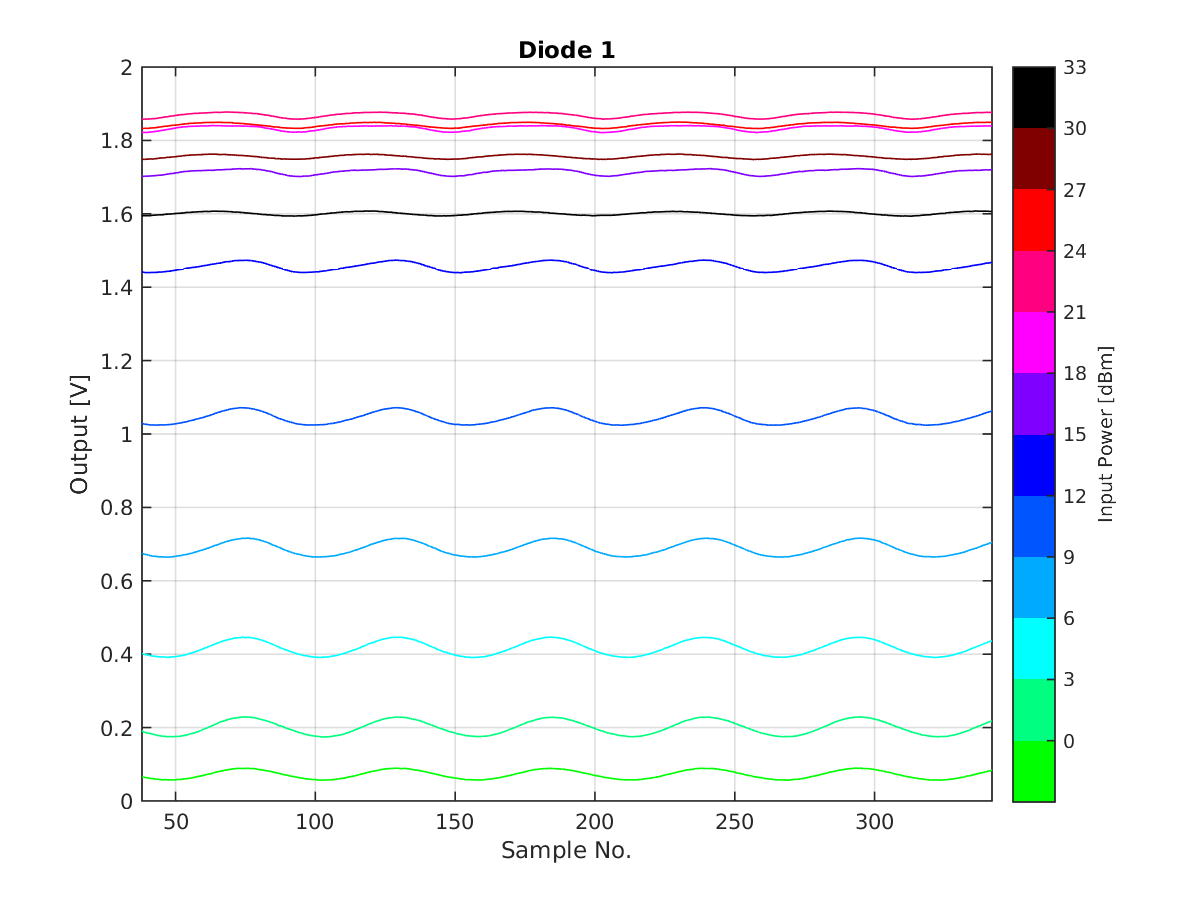
\includegraphics[width=0.9\textwidth]{Figures/phaseMons/Diode1_AllPowerLevels}
  \caption{Response of Diode 1 to signal generator input.}
  \label{f:sigGenAllDio1}
\end{figure}

\begin{figure}
  \centering
  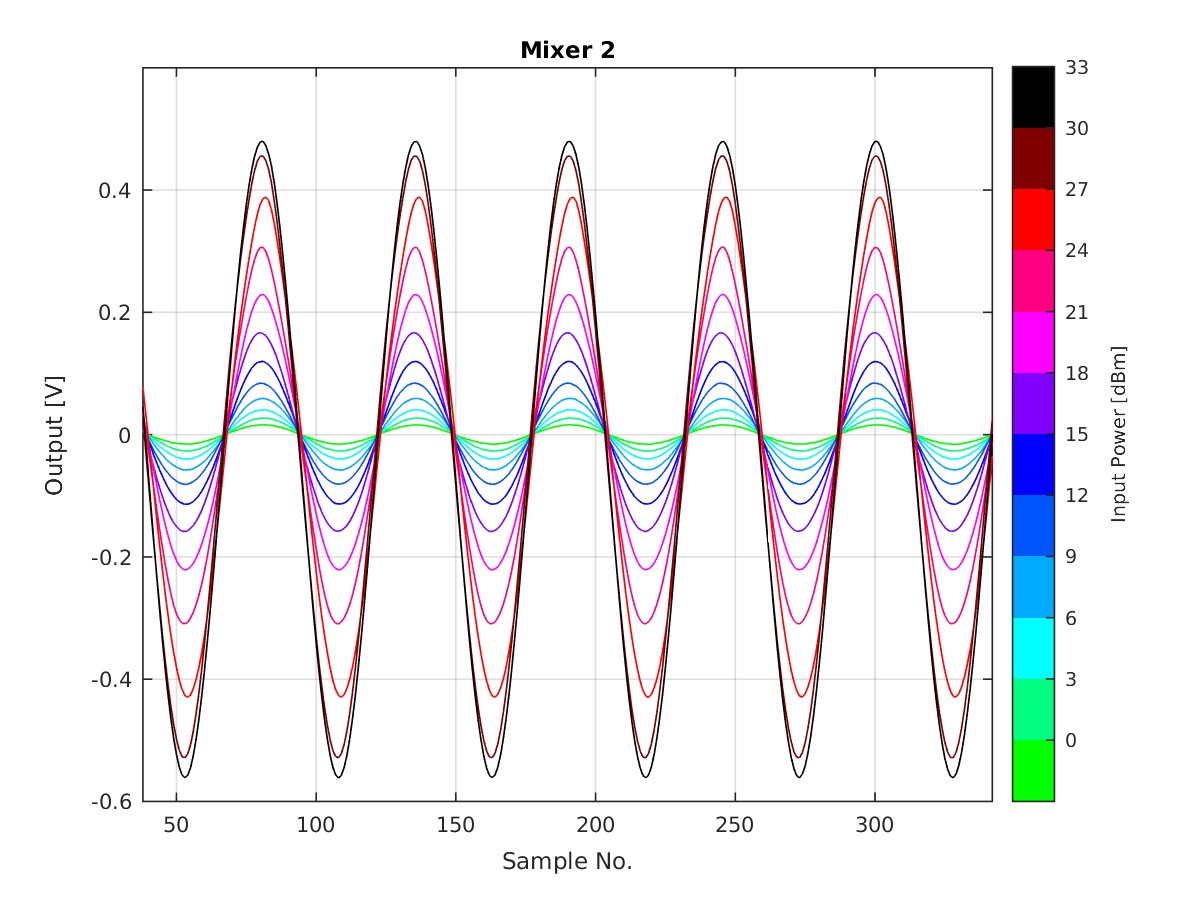
\includegraphics[width=0.9\textwidth]{Figures/phaseMons/Mixer2_AllPowerLevels}
  \caption{Response of Mixer 2 to signal generator input.}
  \label{f:sigGenAllMix2}
  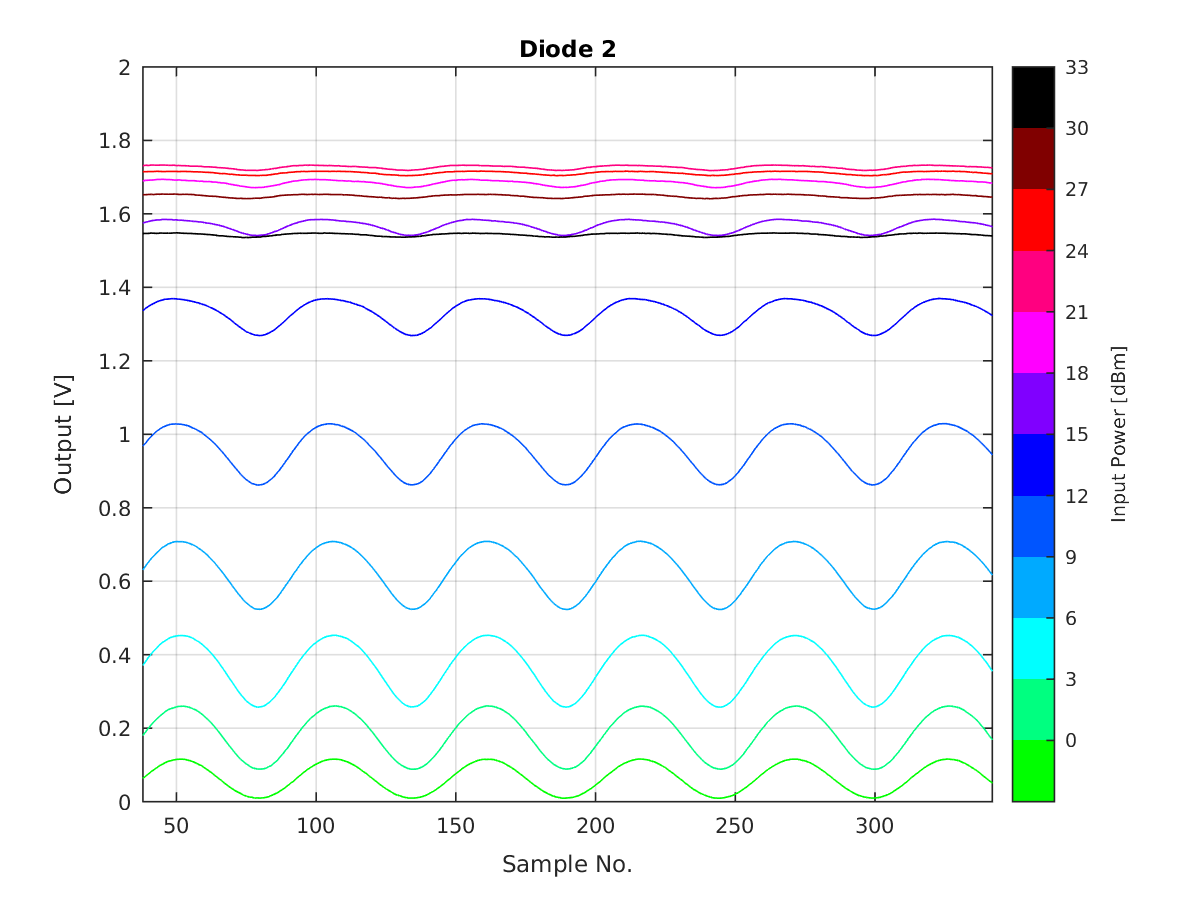
\includegraphics[width=0.9\textwidth]{Figures/phaseMons/Diode2_AllPowerLevels}
  \caption{Response of Diode 2 to signal generator input.}
  \label{f:sigGenAllDio2}
\end{figure}

\begin{figure}
  \centering
  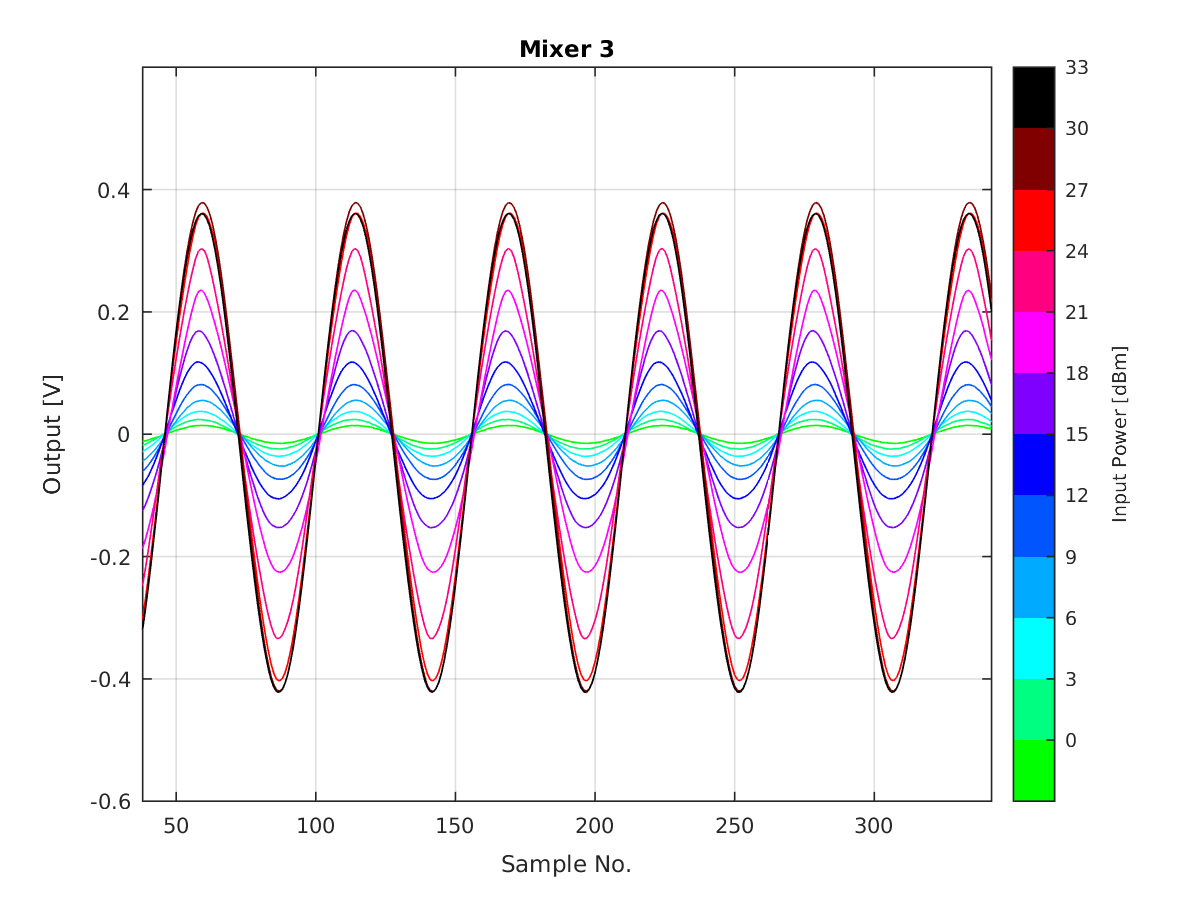
\includegraphics[width=0.9\textwidth]{Figures/phaseMons/Mixer3_AllPowerLevels}
  \caption{Response of Mixer 3 to signal generator input.}
  \label{f:sigGenAllMix3}
  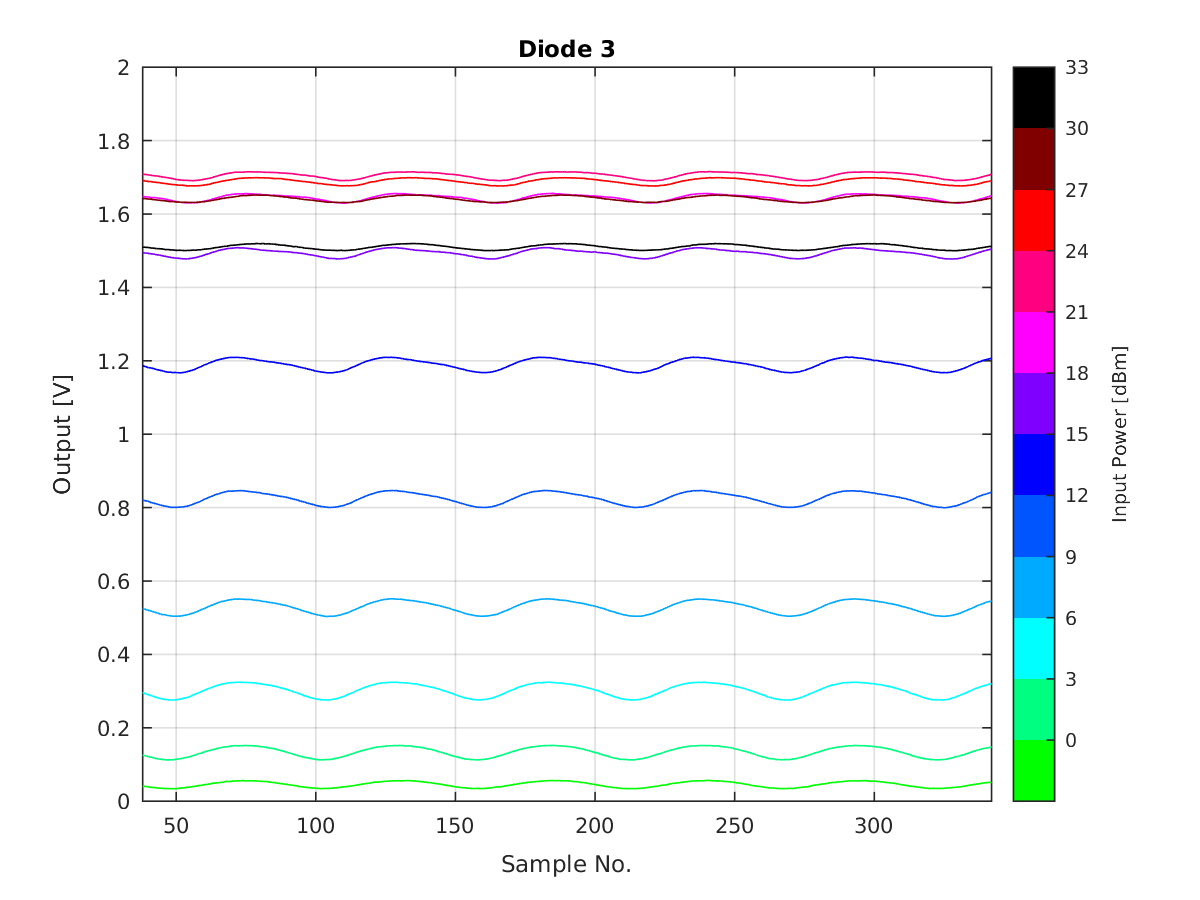
\includegraphics[width=0.9\textwidth]{Figures/phaseMons/Diode3_AllPowerLevels}
  \caption{Response of Diode 3 to signal generator input.}
  \label{f:sigGenAllDio3}
\end{figure}

\subsection{Mixer Response}
\label{ss:sigGenMixFit}

Figure~\ref{f:mixersFit27dBm} shows fits to the response of all mixer outputs at an input power of 27~dBm, close to the typical input power from the beam signals when they are connected. Markers show the data points and the lines are sine fits to the data. The phase offset (displacement in peaks) between the output of each mixer holds no significance for the electronics performance. This is set only by the relative phase between the signal generator and the LO at the time the measurement was started. For normal operation with beam the LO phase shifters are changed to match the phasing of each set of electronics (Section~\ref{s:monCalibrations}).

The reconstruction of the phase from the mixer output depends on the mixer output being sinusoidal. In particular the maximum mixer output, or equivalently the gradient around zero mixer output (using the small angle approximation) is critical due to the dependence on the amplitude in Equation~\ref{e:phaseRecIdeal}. Each set of electronics has a different output amplitude due to slight differences in the LO power for each set of electronics and between the individual components used. At an input power of 27~dBm Mixer 1 has a higher peak output of 510~mV, compared to 410~mV and 380~mV for Mixer 2 and Mixer 3 respectively. 

Overall, the agreement between the actual mixer output and the sinusoidal fits at this input power is good. However, there is some distortion away from the ideal sine curve that is most visible around the maximum and minimum mixer output. Figure~\ref{f:mixersFitResid27dBm} shows the residuals between the mixer outputs and the sine fits across one half wavelength -- from maximum output to minimum output. In the figure the plotted residual is the difference between the fit and the data expressed in terms of an equivalent phase offset, \(\Delta \phi\), using:
\begin{equation}
\Delta \phi(t) = \arcsin\left(\frac{V_{MIXER}(t)-V_{FIT}(t)}{A}\right)
\end{equation}
Where \(V_{MIXER}(t)\) and \(V_{FIT}(t)\) are the mixer voltage and fitted voltage at sample \(t\) respectively, and \(A\) is the fitted mixer amplitude. On the falling slope between the peaks there is only a slight oscillation about the ideal sinusoidal behaviour. The deviation from ideal is at the level of \(0.25\pm0.03^\circ\) and \(0.30\pm0.04^\circ\) for the first and third mixers, with a slightly larger effect of \(0.45\pm0.04^\circ\) for the second mixer. This applies within \(\pm80^\circ\) of the zero crossing in the mixer output. Within \(\pm10^\circ\) of the maximum or minimum output the deviation from the sine fit rapidly increases, reaching several degrees for each mixer. For operation with the beam this means that the accuracy of the phase measurement cannot be guaranteed when the LO phase is set so that the mixer is giving close to its maximum or minimum output. This is also true for other reasons, as seen in Section~\ref{s:resolution}. The PFF system can only correct small offsets at the level of around \(\pm5^\circ\) (Section~\ref{ss:corrRange}), so the non-ideal response close to peak output is not an issue for the PFF performance.

\begin{figure}
  \centering
  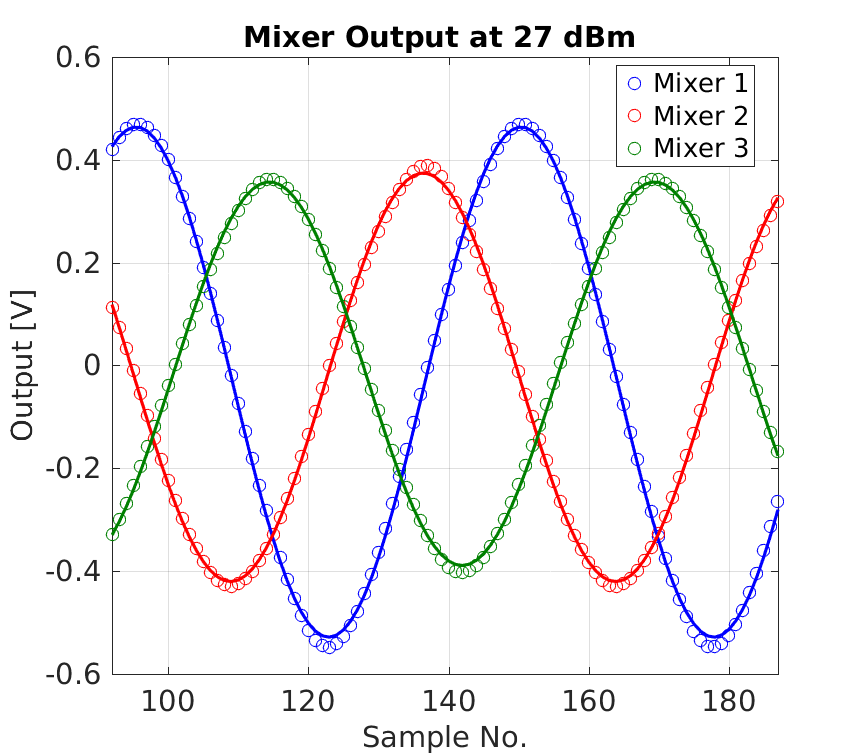
\includegraphics[width=0.9\textwidth]{Figures/phaseMons/mixersFit27dBm}
  \caption{Sinusoidal fit to mixer responses at 27~dBm input power.}
  \label{f:mixersFit27dBm}
\end{figure}

\begin{figure}
  \centering
  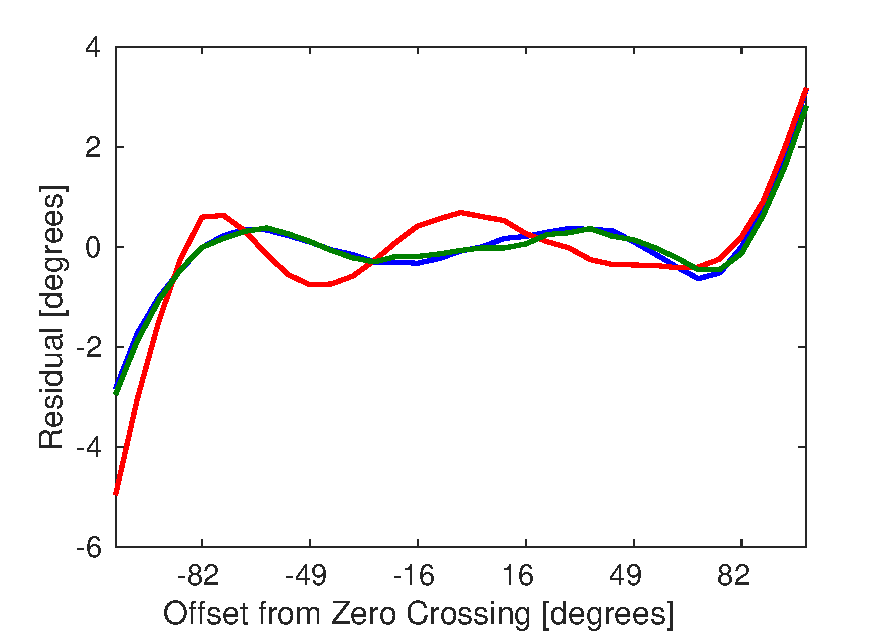
\includegraphics[width=0.9\textwidth]{Figures/phaseMons/mixersFitResid27dBm}
  \caption{Residuals to sinusoidal fit at 27dBm.[TODO: sample numbers don't relate to previous plots]}
  \label{f:mixersFitResid27dBm}
\end{figure}

However, for input powers in the range from 15--21~dBm the non-ideal characteristics of the mixers are larger. One example of this is shown in Figure~\ref{f:mixersFit18dBm}, at an input power of 18~dBm. If input powers in this range are used calibrations of the mixer response should normally be restricted to around the zero crossing so that the fitted amplitude gives the best approximation to the true behaviour for small phase offsets. 

\begin{figure}
  \centering
  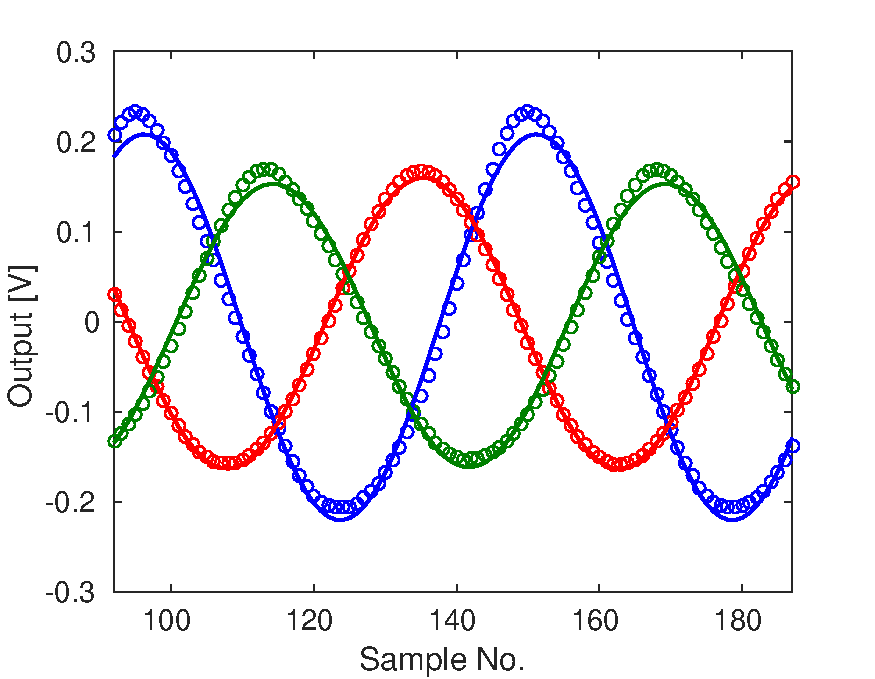
\includegraphics[width=0.9\textwidth]{Figures/phaseMons/mixersFit18dBm}
  \caption{Sinusoidal fit to mixer responses at 18~dBm input power.}
  \label{f:mixersFit18dBm}
\end{figure}

\subsection{Dependence on Input Power}
\label{ss:monSaturation}

The mixer output is expected to linearly depend on the input voltage and the diode on the square of the input voltage. Both these dependencies must hold in order to use Equation~\ref{e:phaseRecIdeal} and obtain a phase measurement that does not depend on the input voltage to the electronics (therefore making the calculated phase insensitive to any possible variations in power along the pulse from the beam signal, for example). For these measurements the input voltage can be calculated using the known input power and 50~\(\Omega\) impedance of the electronics.

Figure~\ref{f:LinFitMixerVsVolts} shows the dependence of the mixer output amplitudes on the input voltage. As seen in the previous section the first mixer gives a larger output than the other two mixers. The 2nd and 3rd mixers give a similar response up to an input voltage of 3.5~V (24~dBm). Dashed lines in the figure show a linear fit to the mixer output restricted to the range between 0.45~V and 1.75~V (6~dBm to 18~dBm) in each case, as marked by the vertical black lines. All three mixers give a linear response up to an input voltage of around 3~V (23~dBm), after which the effects of saturation begin to appear. By an input voltage of 5~V (27~dBm) the first and third mixers are almost fully saturated with almost no remaining power dependence in the output. The second mixer begins to enter saturation at the same voltage as the other two mixers but retains a strong power dependence up to a higher input voltage of 7~V (30~dBm).

\begin{figure}
  \centering
  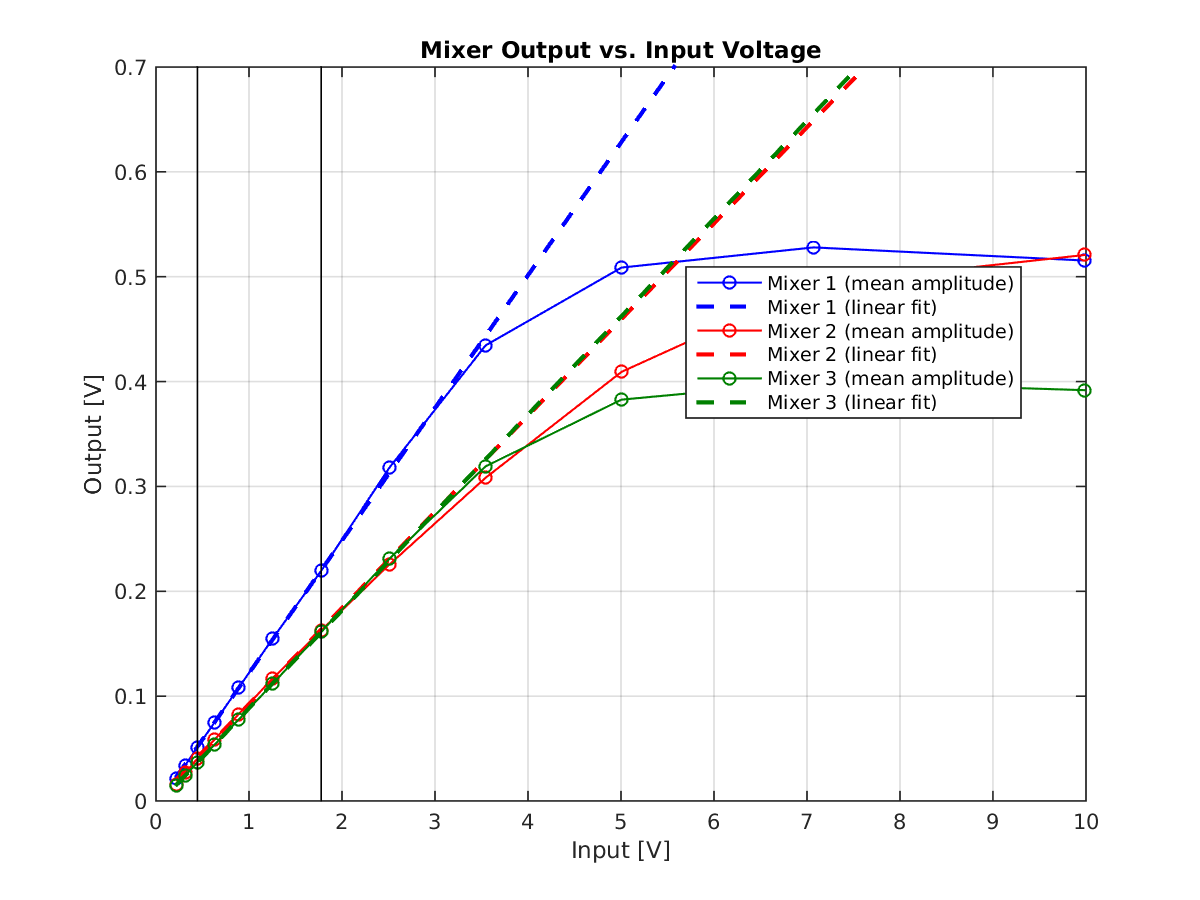
\includegraphics[width=0.9\textwidth]{Figures/phaseMons/LinFitMixerVsVolts}
  \caption{Linear fit to mixer output voltage vs. input voltage.}
  \label{f:LinFitMixerVsVolts}
\end{figure}

The equivalent result for the three diode outputs is shown in Figure~\ref{f:SqrtDiodeVsVolts}, with the square root of the diode output plotted rather than the diode directly as this is the expected linear relationship. Immediately it is apparent that the diode signals saturate at much lower input voltages than the mixer signals. All three diodes are almost fully saturated at an input of 2~V (20~dBm), with the effects of saturation already beginning to appear above 1.25~V (15~dBm). Figure~\ref{f:LinFitSqrtDiodeVsVolts} shows a linear fit to the square root of the diode, using the range of input voltages between 0.45~V and 1.25~V (6--15~dBm). Even below saturation the response of sqrt(Diode) is not well approximated by a linear dependence as desired. However, in the range from 0.30~V 1.25~V (3~dBm to 15~dBm) a quadratic fit to the diode output directly (not sqrt(Diode)) does give a good approximation to the true dependence of the diodes on the input voltage. This is shown in Figure~\ref{f:QuadFitDiodeVsVolts}.

\begin{figure}
  \centering
  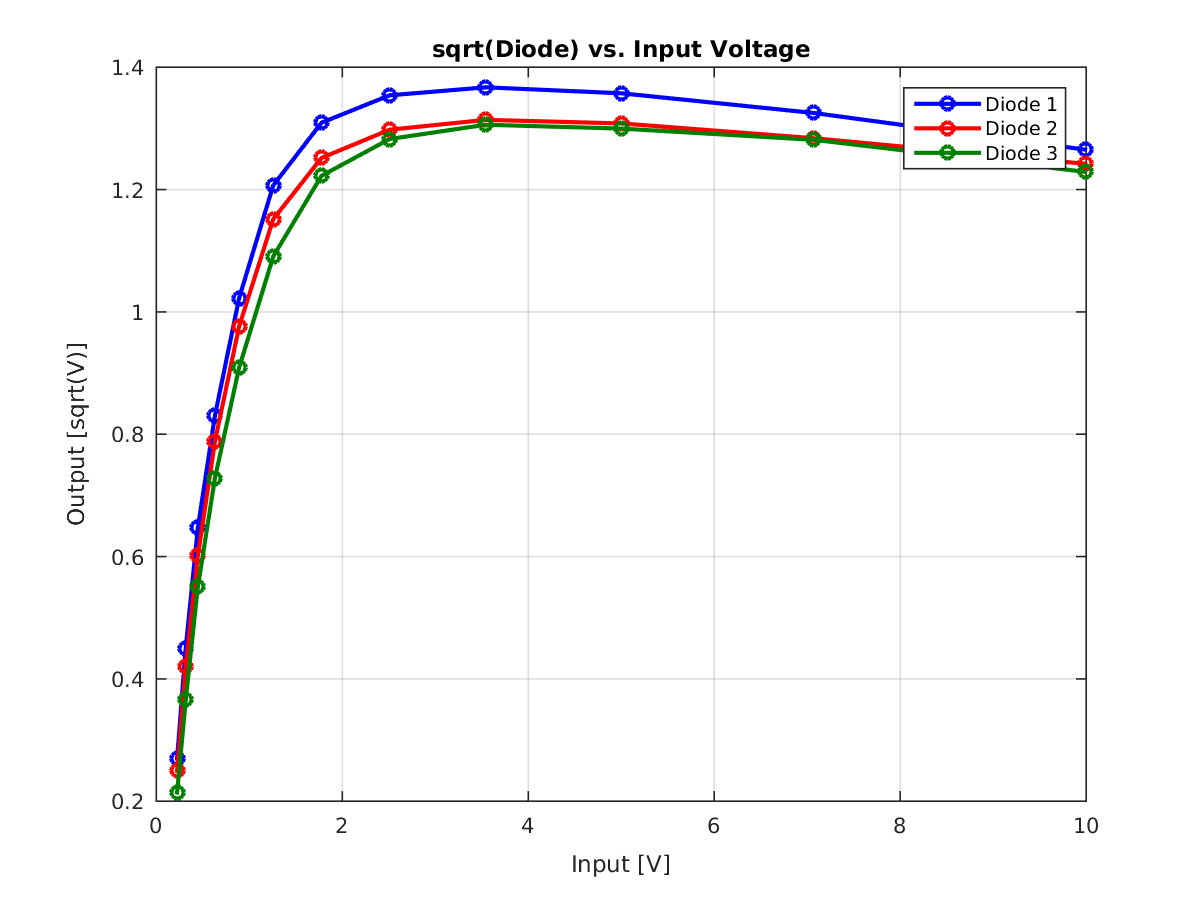
\includegraphics[width=0.9\textwidth]{Figures/phaseMons/SqrtDiodeVsVolts}
  \caption{sqrt(Diode) vs. input voltage.}
  \label{f:SqrtDiodeVsVolts}
\end{figure}

\begin{figure}
  \centering
  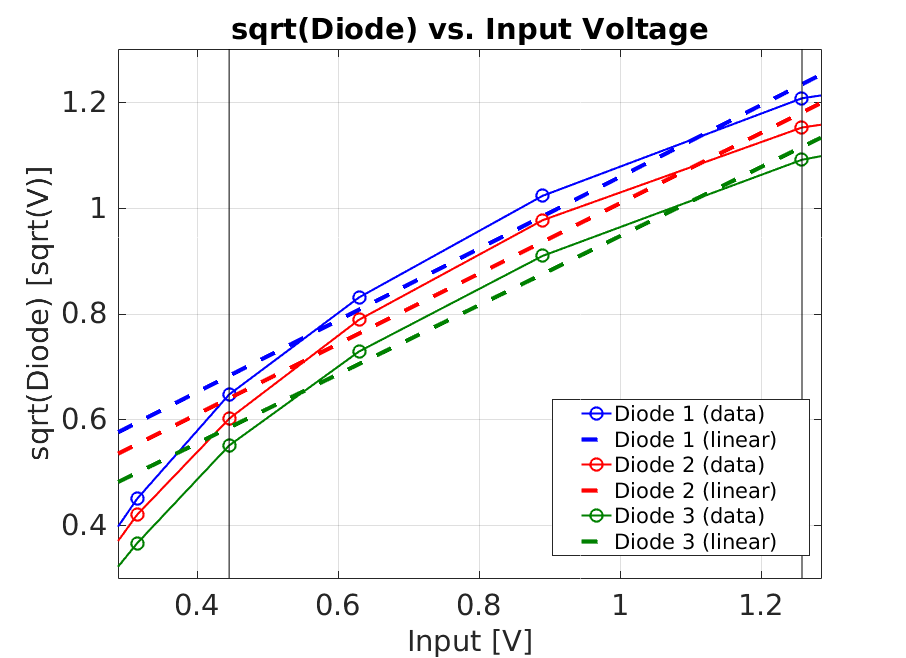
\includegraphics[width=0.9\textwidth]{Figures/phaseMons/LinFitSqrtDiodeVsVolts}
  \caption{Linear fits to sqrt(Diode) vs. input voltage.}
  \label{f:LinFitSqrtDiodeVsVolts}
  \centering
  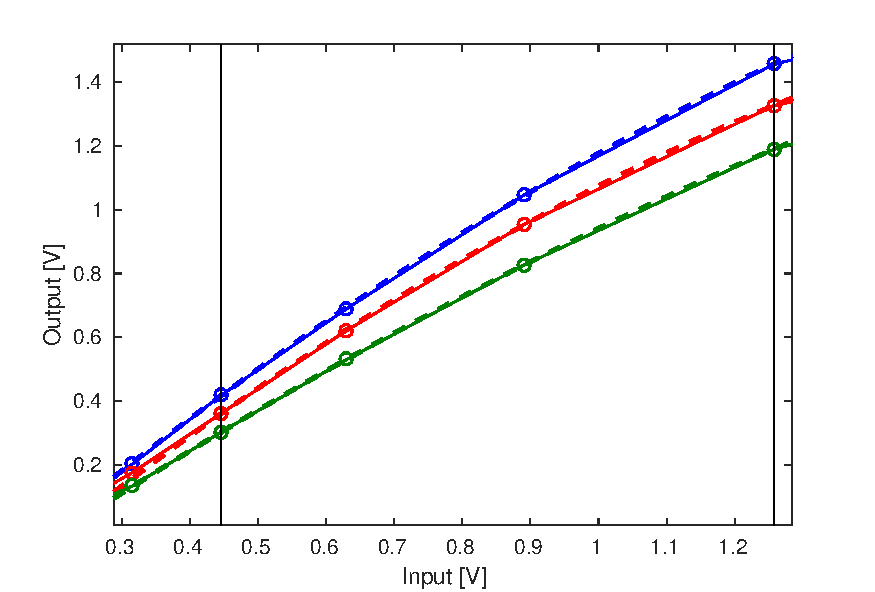
\includegraphics[width=0.9\textwidth]{Figures/phaseMons/QuadFitDiodeVsVolts}
  \caption{Quadratic fits to Diode vs. input voltage.}
  \label{f:QuadFitDiodeVsVolts}
\end{figure}


\subsection{Cross-Talk}
\label{ss:crossTalk}



\begin{figure}
  \centering
  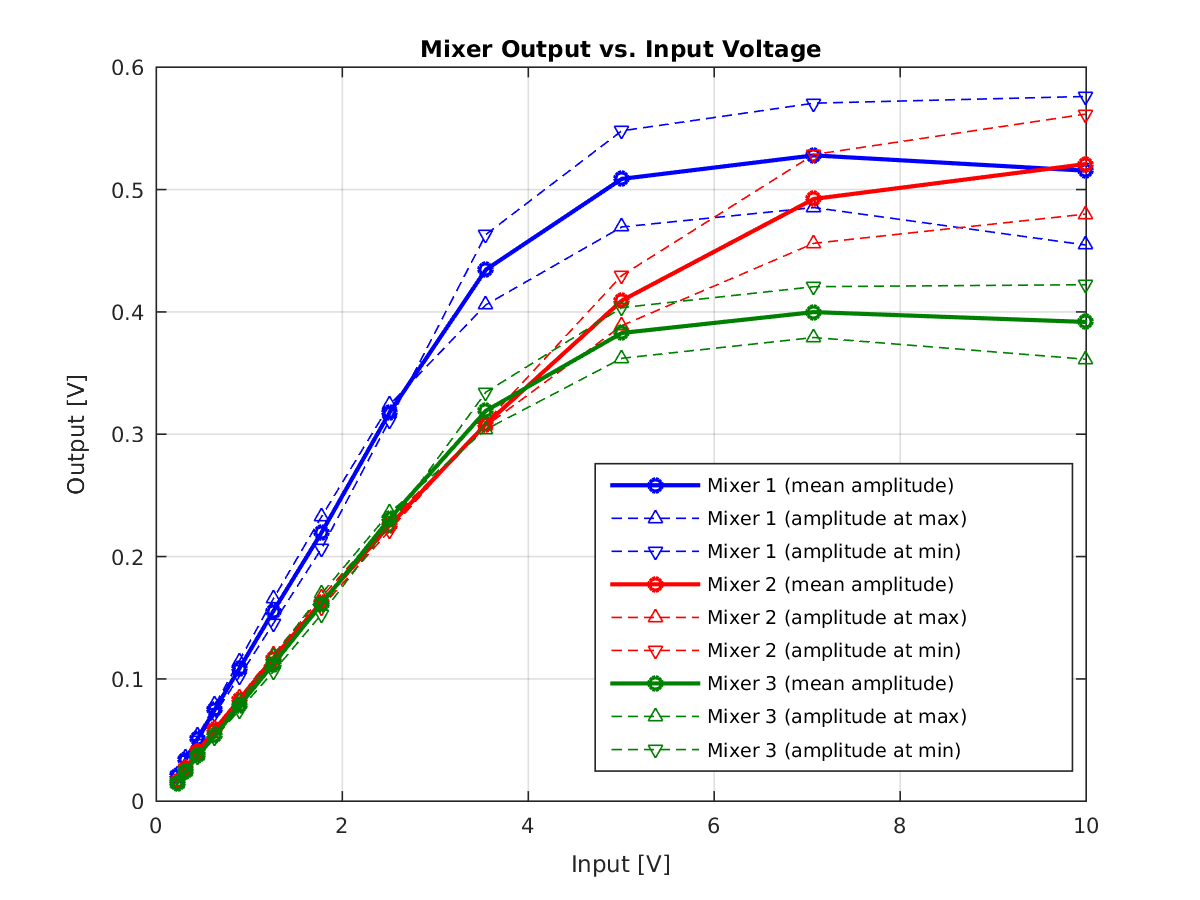
\includegraphics[width=0.9\textwidth]{Figures/phaseMons/MixerVsVolts}
  \caption{Mixer output voltage vs. input voltage.}
  \label{f:MixerVsVolts}
\end{figure}

\begin{figure}
  \centering
  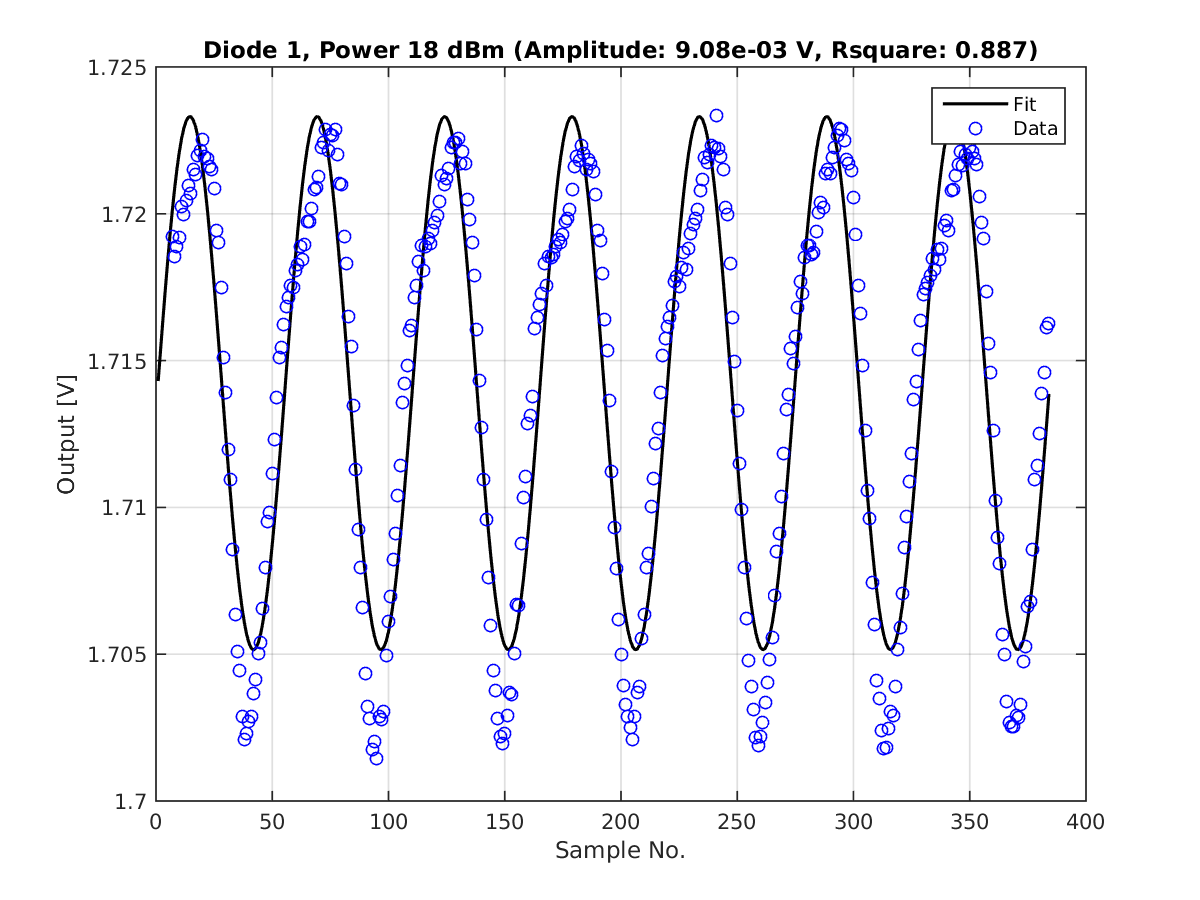
\includegraphics[width=0.9\textwidth]{Figures/phaseMons/Diode1_Power18}
  \caption{Sinusoidal fit to cross-talk on diode at 18~dBm input power.}
  \label{f:Diode1_Power18}
\end{figure}

\begin{figure}
  \centering
  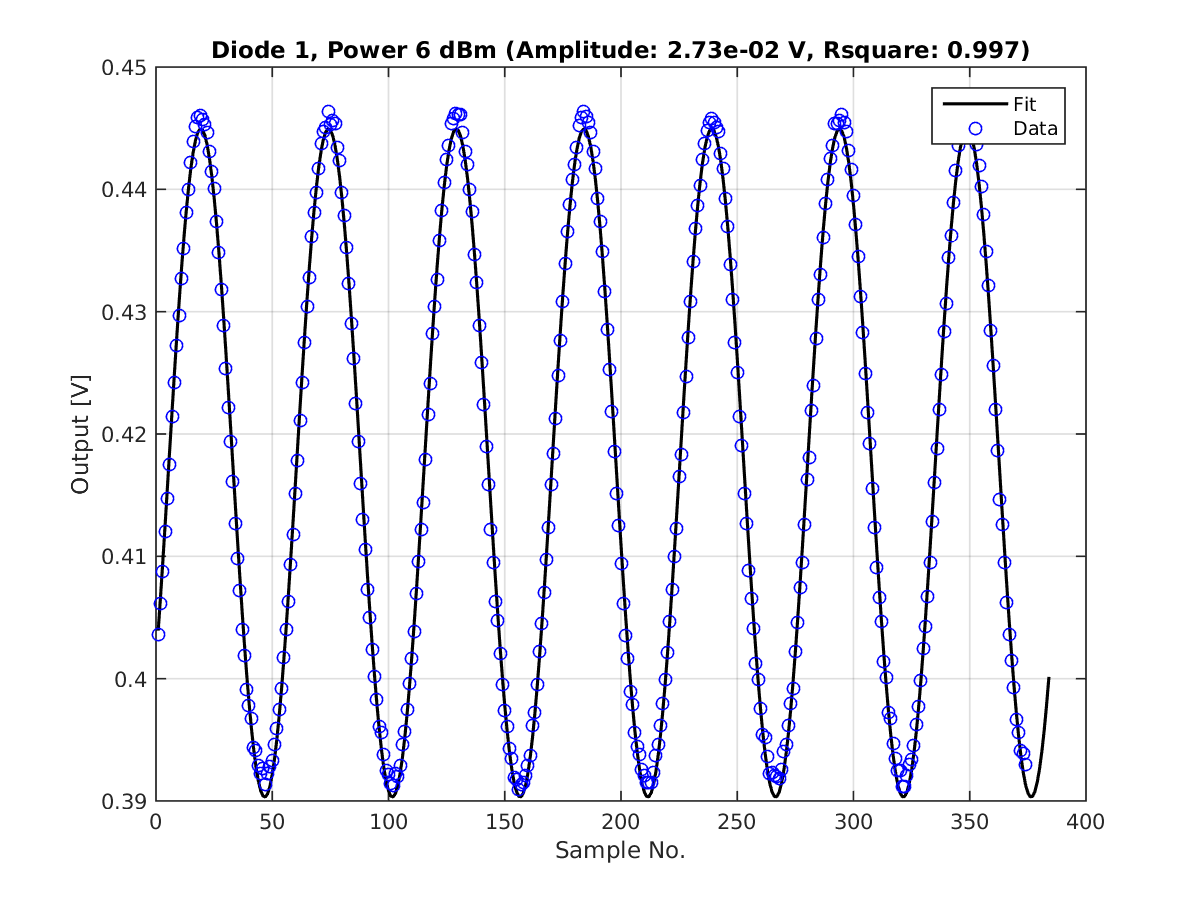
\includegraphics[width=0.9\textwidth]{Figures/phaseMons/Diode1_Power6}
  \caption{Sinusoidal fit to cross-talk on diode at 6~dBm input power.}
  \label{f:Diode1_Power6}
\end{figure}

\begin{figure}
  \centering
  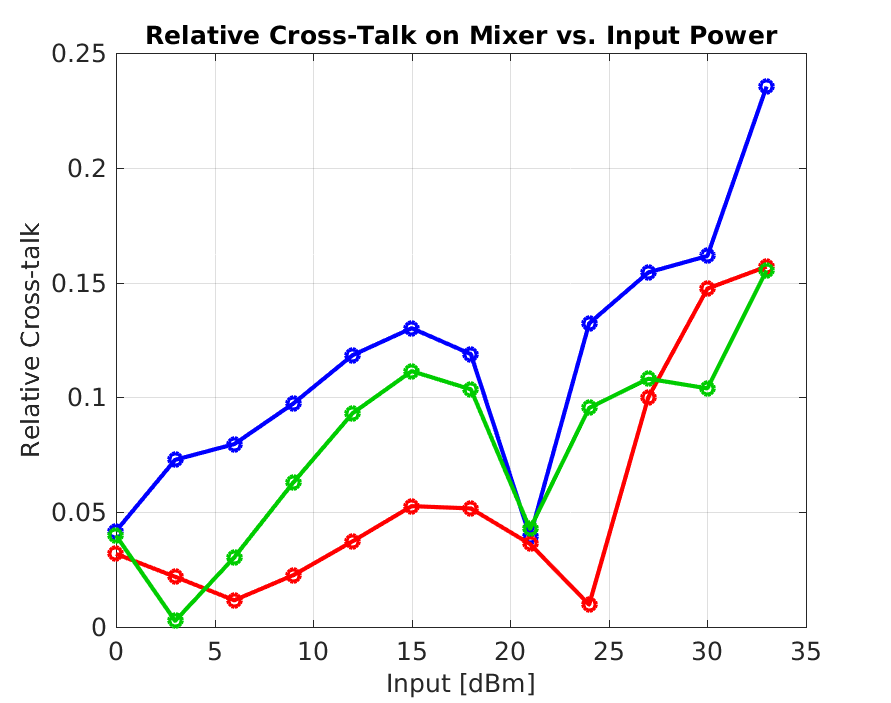
\includegraphics[width=0.9\textwidth]{Figures/phaseMons/RelativeMixerXTalkvsPower}
  \caption{Relative amplitude vs. input power of cross-talk on the mixer from the diode.}
  \label{f:RelativeMixerXTalkvsPower}
\end{figure}

\begin{figure}
  \centering
  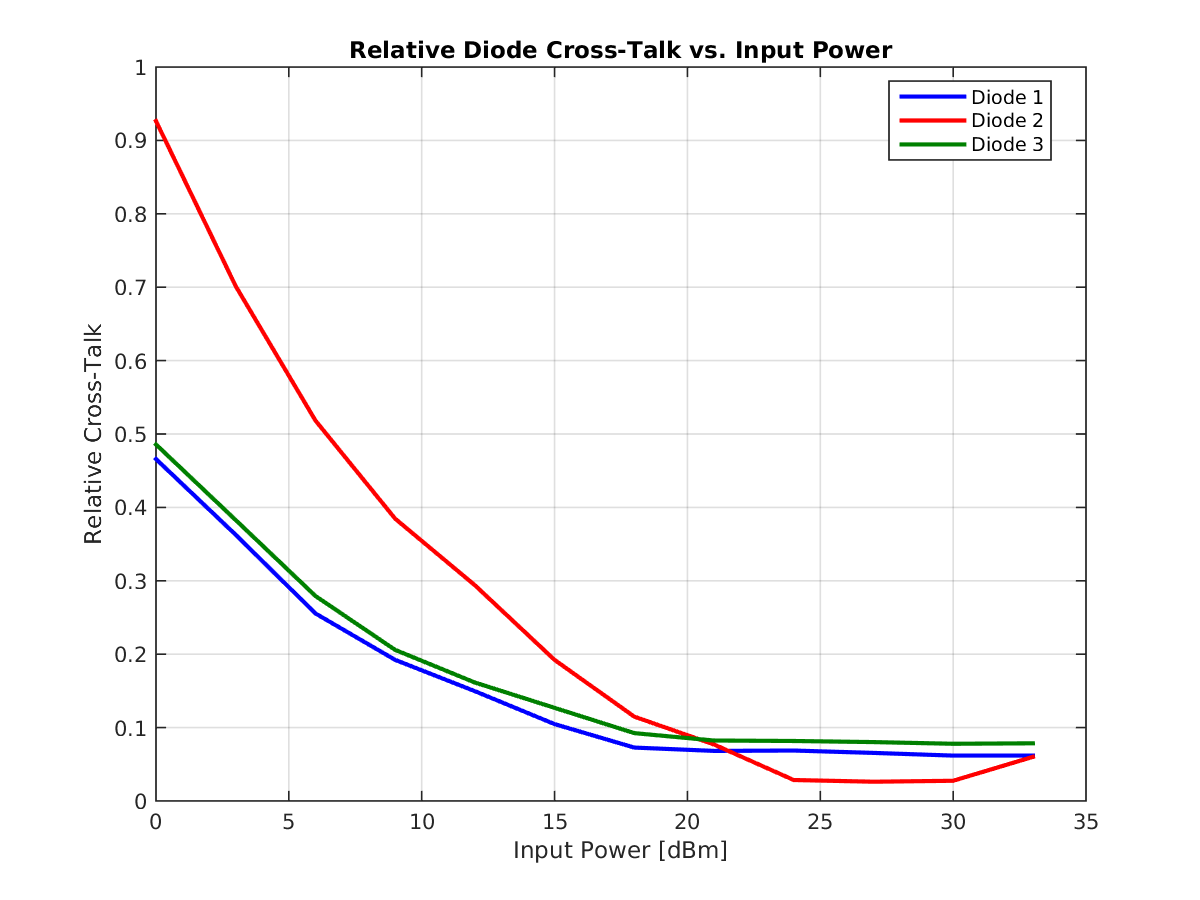
\includegraphics[width=0.9\textwidth]{Figures/phaseMons/RelativeDiodeXTalkVsPower}
  \caption{Relative amplitude vs. input power of cross-talk on the diode from the mixer.}
  \label{f:RelativeDiodeXTalkVsPower}
\end{figure}

\newsection{monCalibrations}{Calibrations}

\subsection{Procedure}
\label{ss:calProcedure}

\subsection{Single Sample Results}
\label{ss:calSingSamp}

\subsection{Multi-Sample Results}
\label{ss:calMultiSamp}

\newsection{digNoise}{Digitiser Noise}

\subsection{On FONT5 Board}
\label{ss:font5Noise}

\subsection{On SiS Digitiser}
\label{ss:sisNoise}

\newsection{shifters}{Phase Shifter Noise}

\subsection{Digital Phase Shifters}
\label{ss:digShiftNoise}

\begin{figure}
  \centering
  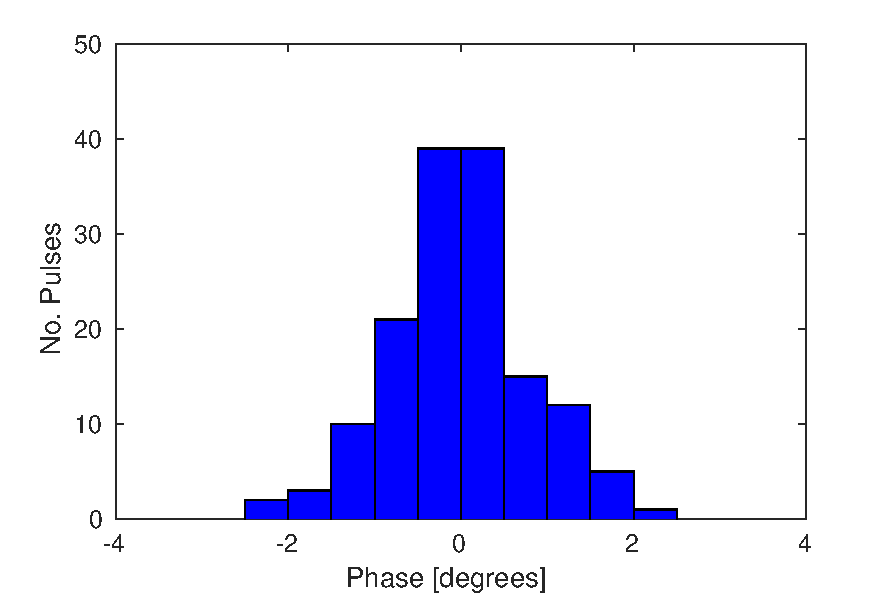
\includegraphics[width=0.9\textwidth]{Figures/phaseMons/PhMon_HistDig1}
  \caption{Dig shifter 1.}
  \label{f:PhMon_HistDig1}
\end{figure}

\begin{figure}
  \centering
  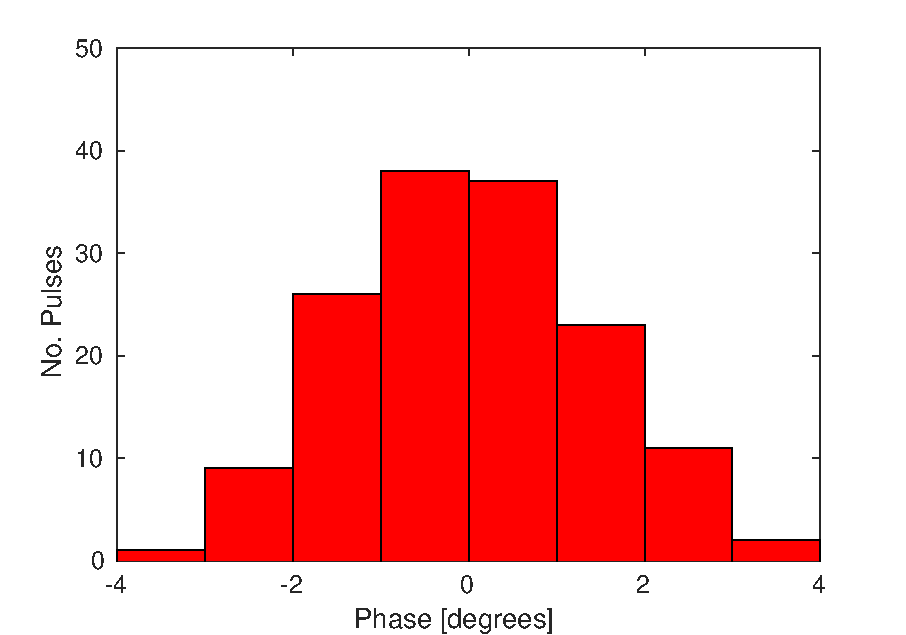
\includegraphics[width=0.9\textwidth]{Figures/phaseMons/PhMon_HistDig2}
  \caption{Dig shifter 2.}
  \label{f:PhMon_HistDig2}
\end{figure}

\begin{figure}
  \centering
  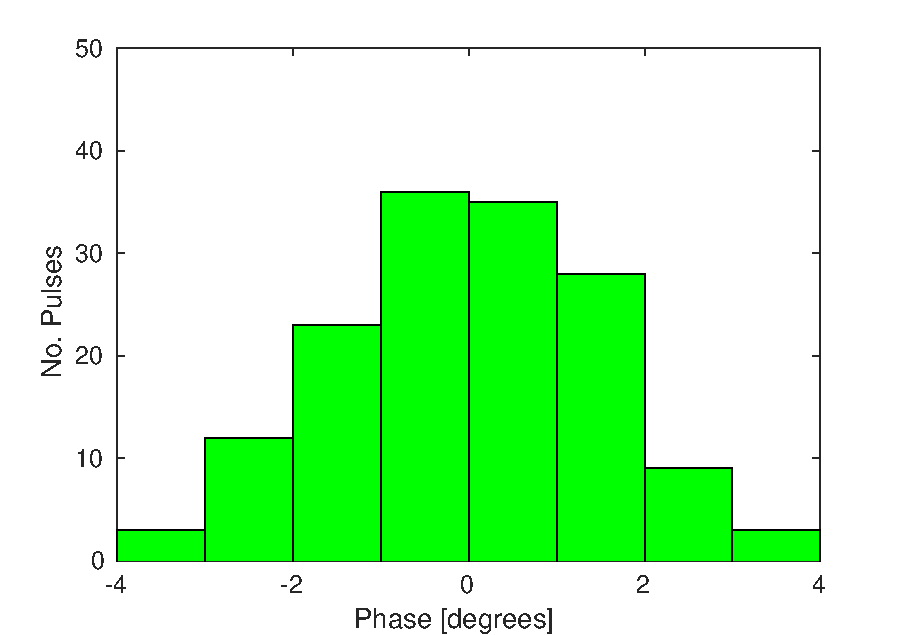
\includegraphics[width=0.9\textwidth]{Figures/phaseMons/PhMon_HistDig3}
  \caption{Dig shifter 3.}
  \label{f:PhMon_HistDig3}
\end{figure}

\subsection{Mechanical Phase Shifters}
\label{ss:mechShiftNoise}

\begin{figure}
  \centering
  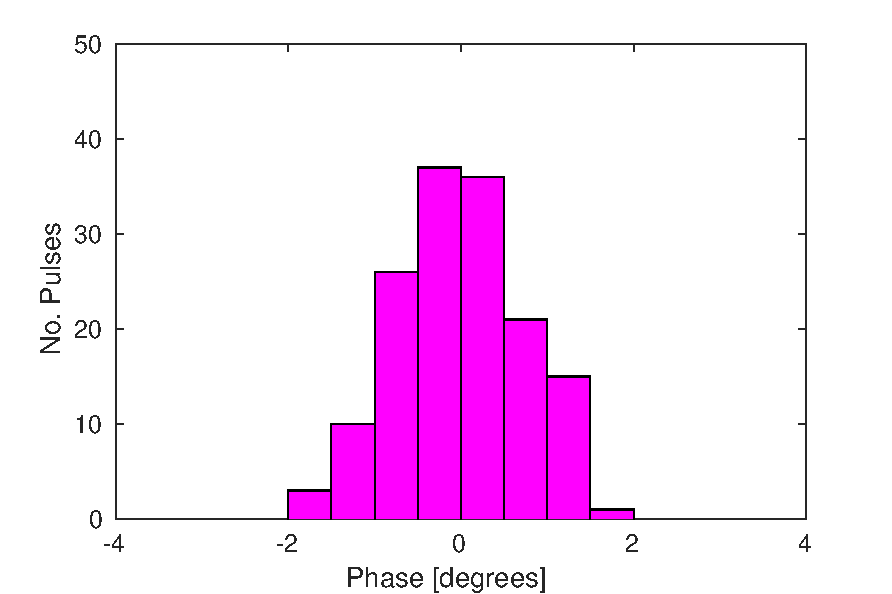
\includegraphics[width=0.9\textwidth]{Figures/phaseMons/PhMon_HistMech}
  \caption{Mech shifter.}
  \label{f:PhMon_HistMech}
\end{figure}

\newsection{resolution}{Resolution}

Single sample.

(Multi-sample)

Sample averaging.

Impact for phase correlations.

vs. shifter setting

\begin{figure}
  \centering
  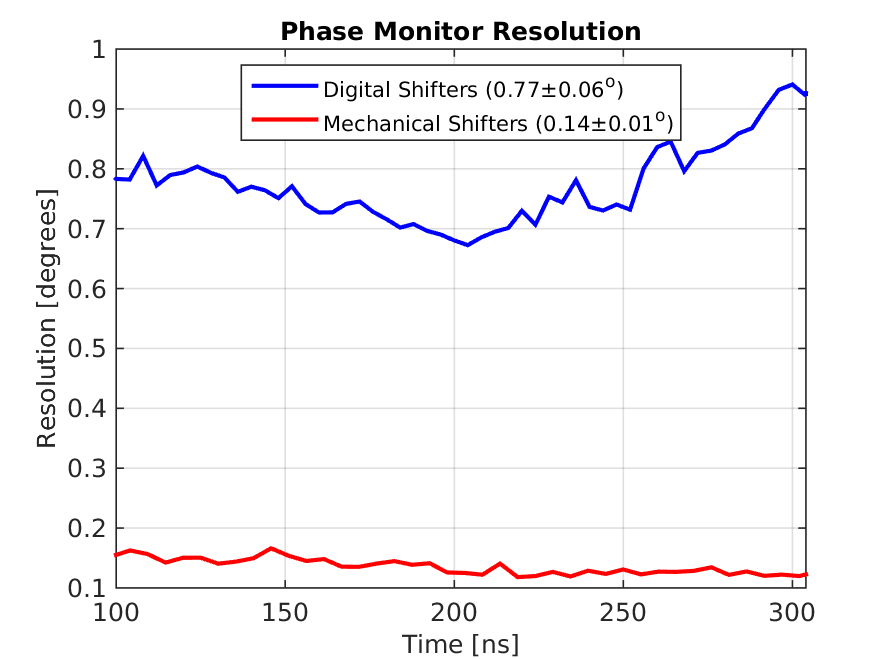
\includegraphics[width=0.9\textwidth]{Figures/phaseMons/PhMon_Resolution}
  \caption{Resolution.}
  \label{f:PhMon_Resolution}
\end{figure}

\newsection{monLinearity}{Linearity}

\newsection{monBandwidth}{Bandwidth}

\newsection{monPosition}{Dependence on Position}








